

%%%
%%%  FIGURE 
%%%
\begin{figure}[h]
\begin{center}
\includegraphics[width=1.\textwidth]{diagrams/bl-exact-meth-upwind.eps}
\end{center}
\caption{Buckley--Leverett test-cases: Saturation solutions for the continuous upwind method for different 1D P$_{1}$DG-P$_{2}$ mesh  resolutions and comparison against standard analytical solution.
\label{bl-exact-meth-upwind}}
\end{figure}

%%%
%%%
%%%  FIGURE 
%%%
\begin{figure}[h]
  %\begin{center}
\vbox{\hbox{\hspace{2.5cm}
    \includegraphics[width=0.62\textwidth]{diagrams/BL_1d_P0DGP1_convergence.eps}}
\vspace{-.0cm}\hbox{\hspace{2.5cm}
    \includegraphics[width=0.62\textwidth]{diagrams/BL_1d_P1DGP2_convergence.eps}}
\vspace{-.0cm}\hbox{\hspace{2.5cm}
    \includegraphics[width=0.62\textwidth]{diagrams/BL_1d_P2DGP3_convergence.eps}}}
   % 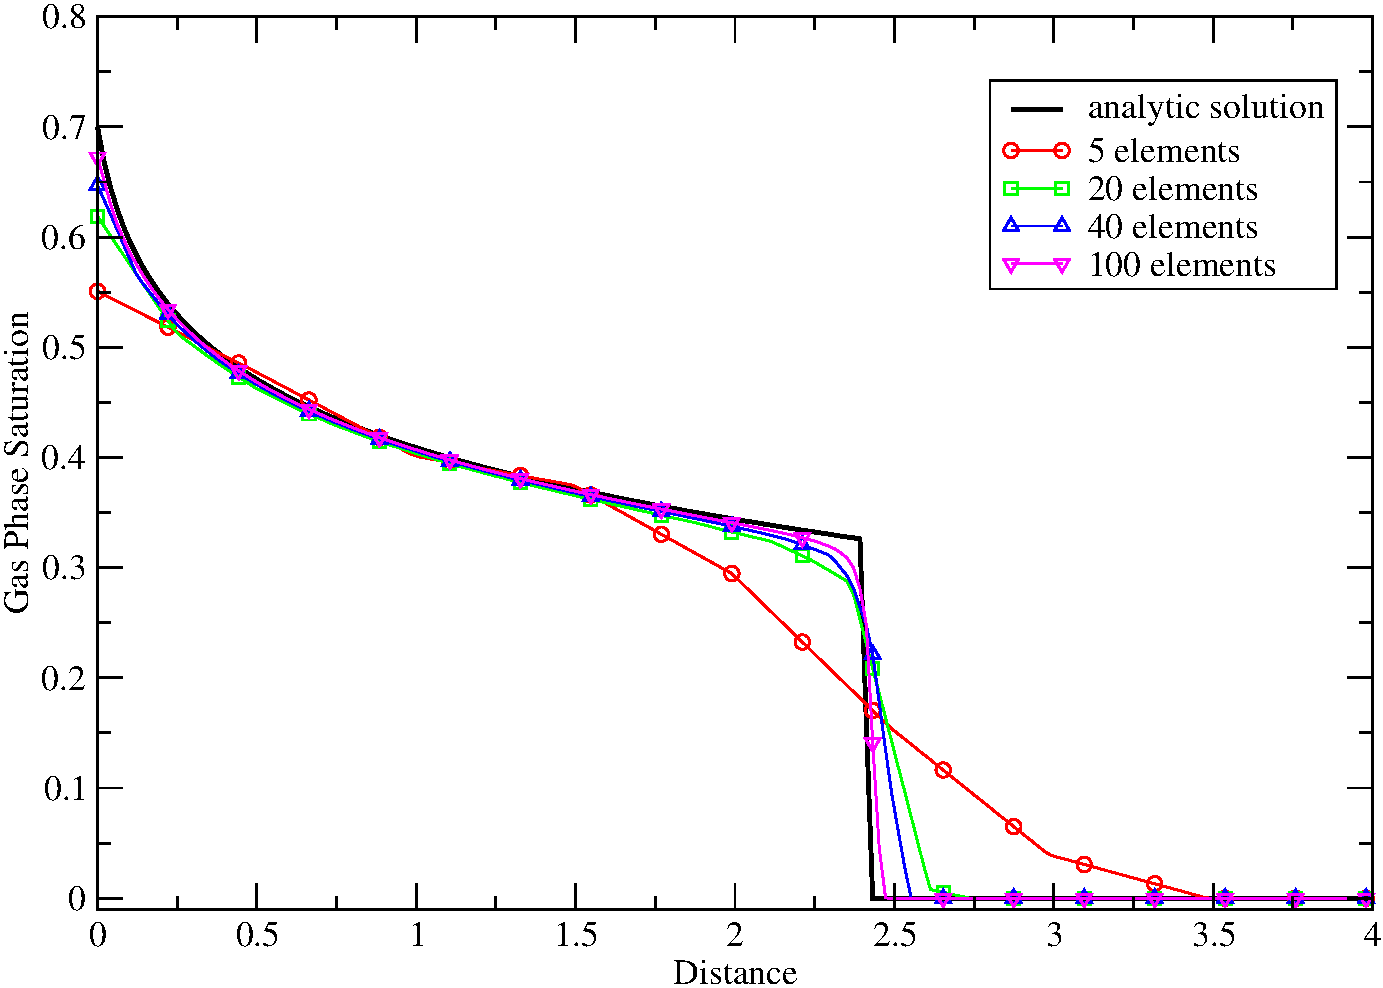
\includegraphics[width=0.45\textwidth]{BL_2d_P1DGP2_convergence}
    \caption{Buckley--Leverett test-cases: Saturation profiles for a number of element-pairs and numerical resolutions in 1D -- P$_{0}$DG-P$_{1}$ (top), P$_{1}$DG-P$_{2}$ and P$_{2}$DG-P$_{3}$ (bottom).\label{fig:BL_profiles}}
  %\end{center}
\end{figure}

%%%
%%%  FIGURE 
%%%
\begin{figure}[h]
\vbox{\hbox{\hspace{1.cm}
    \includegraphics[width=0.8\textwidth]{diagrams/L1_convergence_rate.eps}}
\vspace{.0cm}\hbox{\hspace{1.cm}
    \includegraphics[width=0.8\textwidth]{diagrams/L2_convergence_rate.eps}}}
    \caption{Buckley--Leverett test-cases: L1 (top) and L2 (bottom) error convergence rates for a number of element pairs. \label{fig:BL_converg-rates}}
\end{figure}

%%%
%%%  FIGURE 
%%%
\begin{figure}[h]
\begin{center}
\includegraphics[width=1.\textwidth]{diagrams/bl-dg-2eles.eps}
\end{center}
\caption{Buckley--Leverett test-cases: Two element solution using the discontinuous formulation. Saturation field from both CV solution and FEM interpolation are shown.  \label{bl-dg-2eles}}
\end{figure}


%%%
%%%  FIGURE 
%%%
\begin{figure}[h]
\vbox{\hbox{\hspace{1.cm}
    \includegraphics[width=0.8\textwidth]{diagrams/L1_convergence_rate_DG.eps}}
\vspace{.0cm}\hbox{\hspace{1.cm}
    \includegraphics[width=0.8\textwidth]{diagrams/L2_convergence_rate_DG.eps}}}
    \caption{Buckley-Leverett test-cases: L1 (top) and L2 (bottom) error convergence rates for a number of fully discontinuous (between elements) element pairs. \label{fig:BL_converg-rates_DG}}
\end{figure}


%%%
%%%  FIGURE 
%%%
\begin{figure}[h]
\vbox{
\hbox{\hspace{.3cm}\includegraphics[width=.9\textwidth]{diagrams/bl-dg-cent-4-10-20.eps}}
\vspace{-0.cm}
\hbox{\hspace{.3cm}\includegraphics[width=.9\textwidth]{diagrams/bl-dg-4-10-20.eps}}}
\caption{Buckley--Leverett test-cases: Saturation field obtained from the discontinuous and continuous formulations with different mesh resolutions. Solutions without (top) and with (bottom) upwinding scheme. Notice that oscillations are suppressed with the upwinding scheme.\label{bl-dg-cent-4-10-20}}
\end{figure}


%%%
%%%  FIGURE 
%%%
\begin{figure}[h]
\vbox{
\hbox{\hspace{.3cm}\includegraphics[width=.9\textwidth]{diagrams/bl-dg-4-10-vers-cty.eps}}
\vspace{-0.cm}
\hbox{\hspace{.3cm}\includegraphics[width=.9\textwidth]{diagrams/bl-dg-p1-2-4-5-10-20-40.eps}}}
\caption{Buckley--Leverett test-cases: Saturation field obtained from (top) continuous and discontinuous (between elements) formulations (solution with 50 elements may be considered as a converged result). Solution obtained (bottom) from linear pressure $\left(\text{P}_{1}\right)$ formulation with different mesh resolution with comparison against P$_{2}$-pressure formulation (continuous). \label{bl-dg-4-10-vers-cty}}
\end{figure}

%%%
%%%  FIGURE 
%%%
\begin{figure}[h]
\vbox{
\hbox{\hspace{.2cm}
    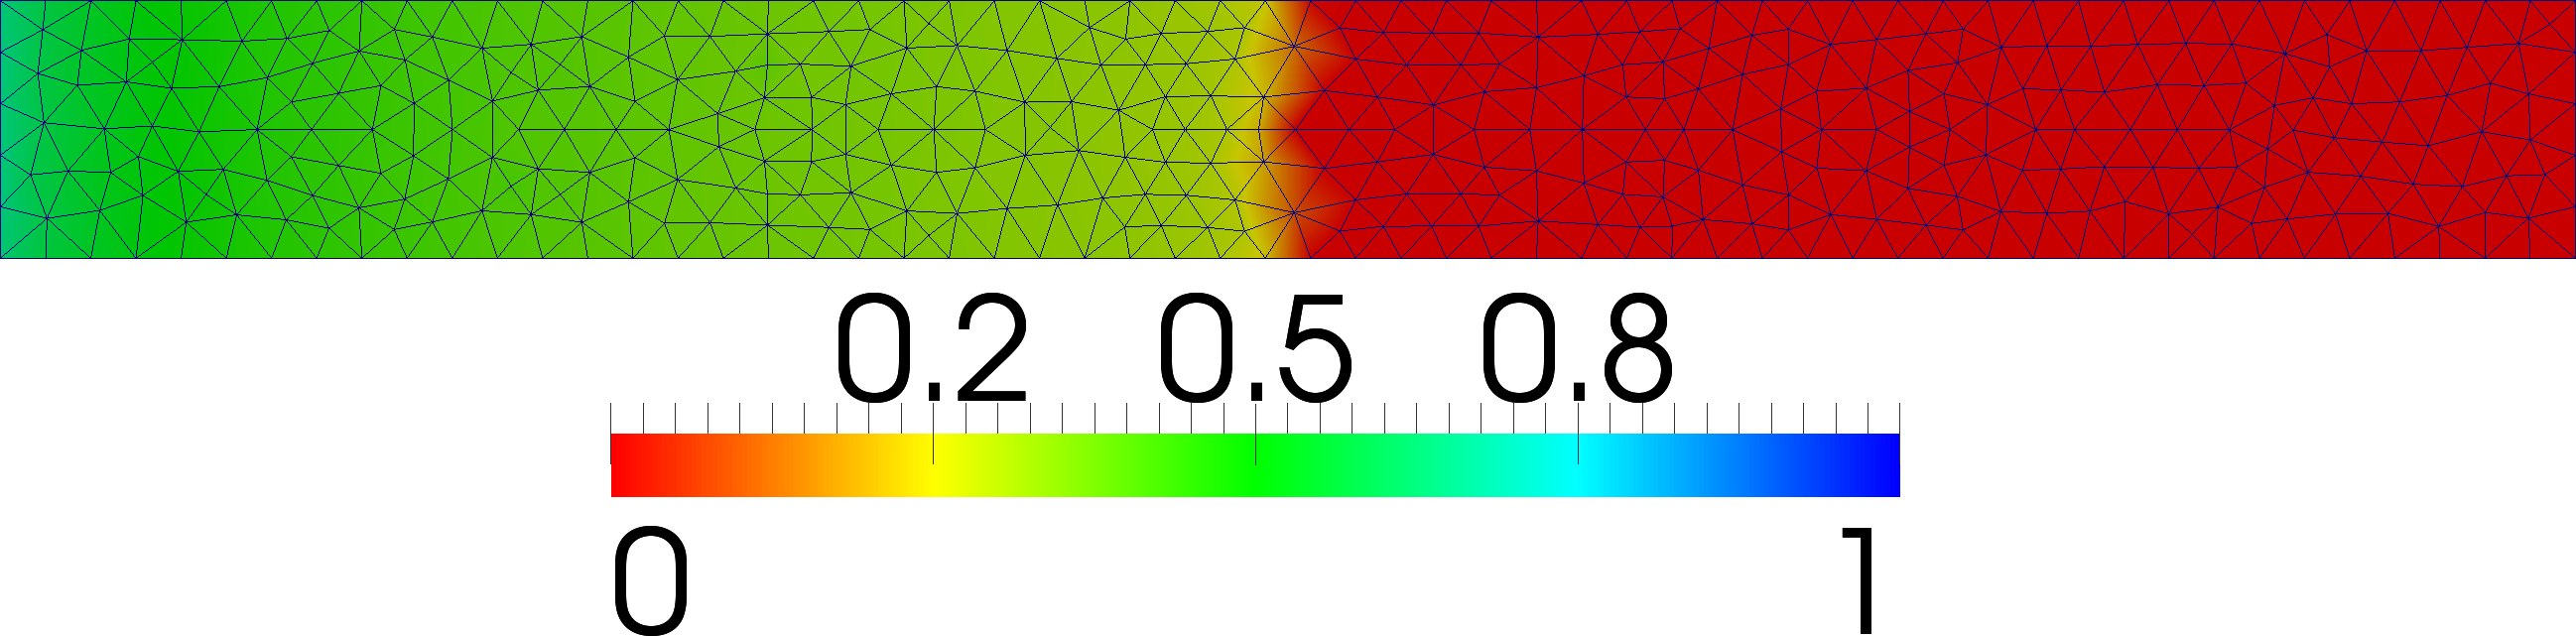
\includegraphics[width=1.\textwidth]{diagrams/map_2d.png}}
\vspace{1.cm}
\hbox{\hspace{0.2cm}
    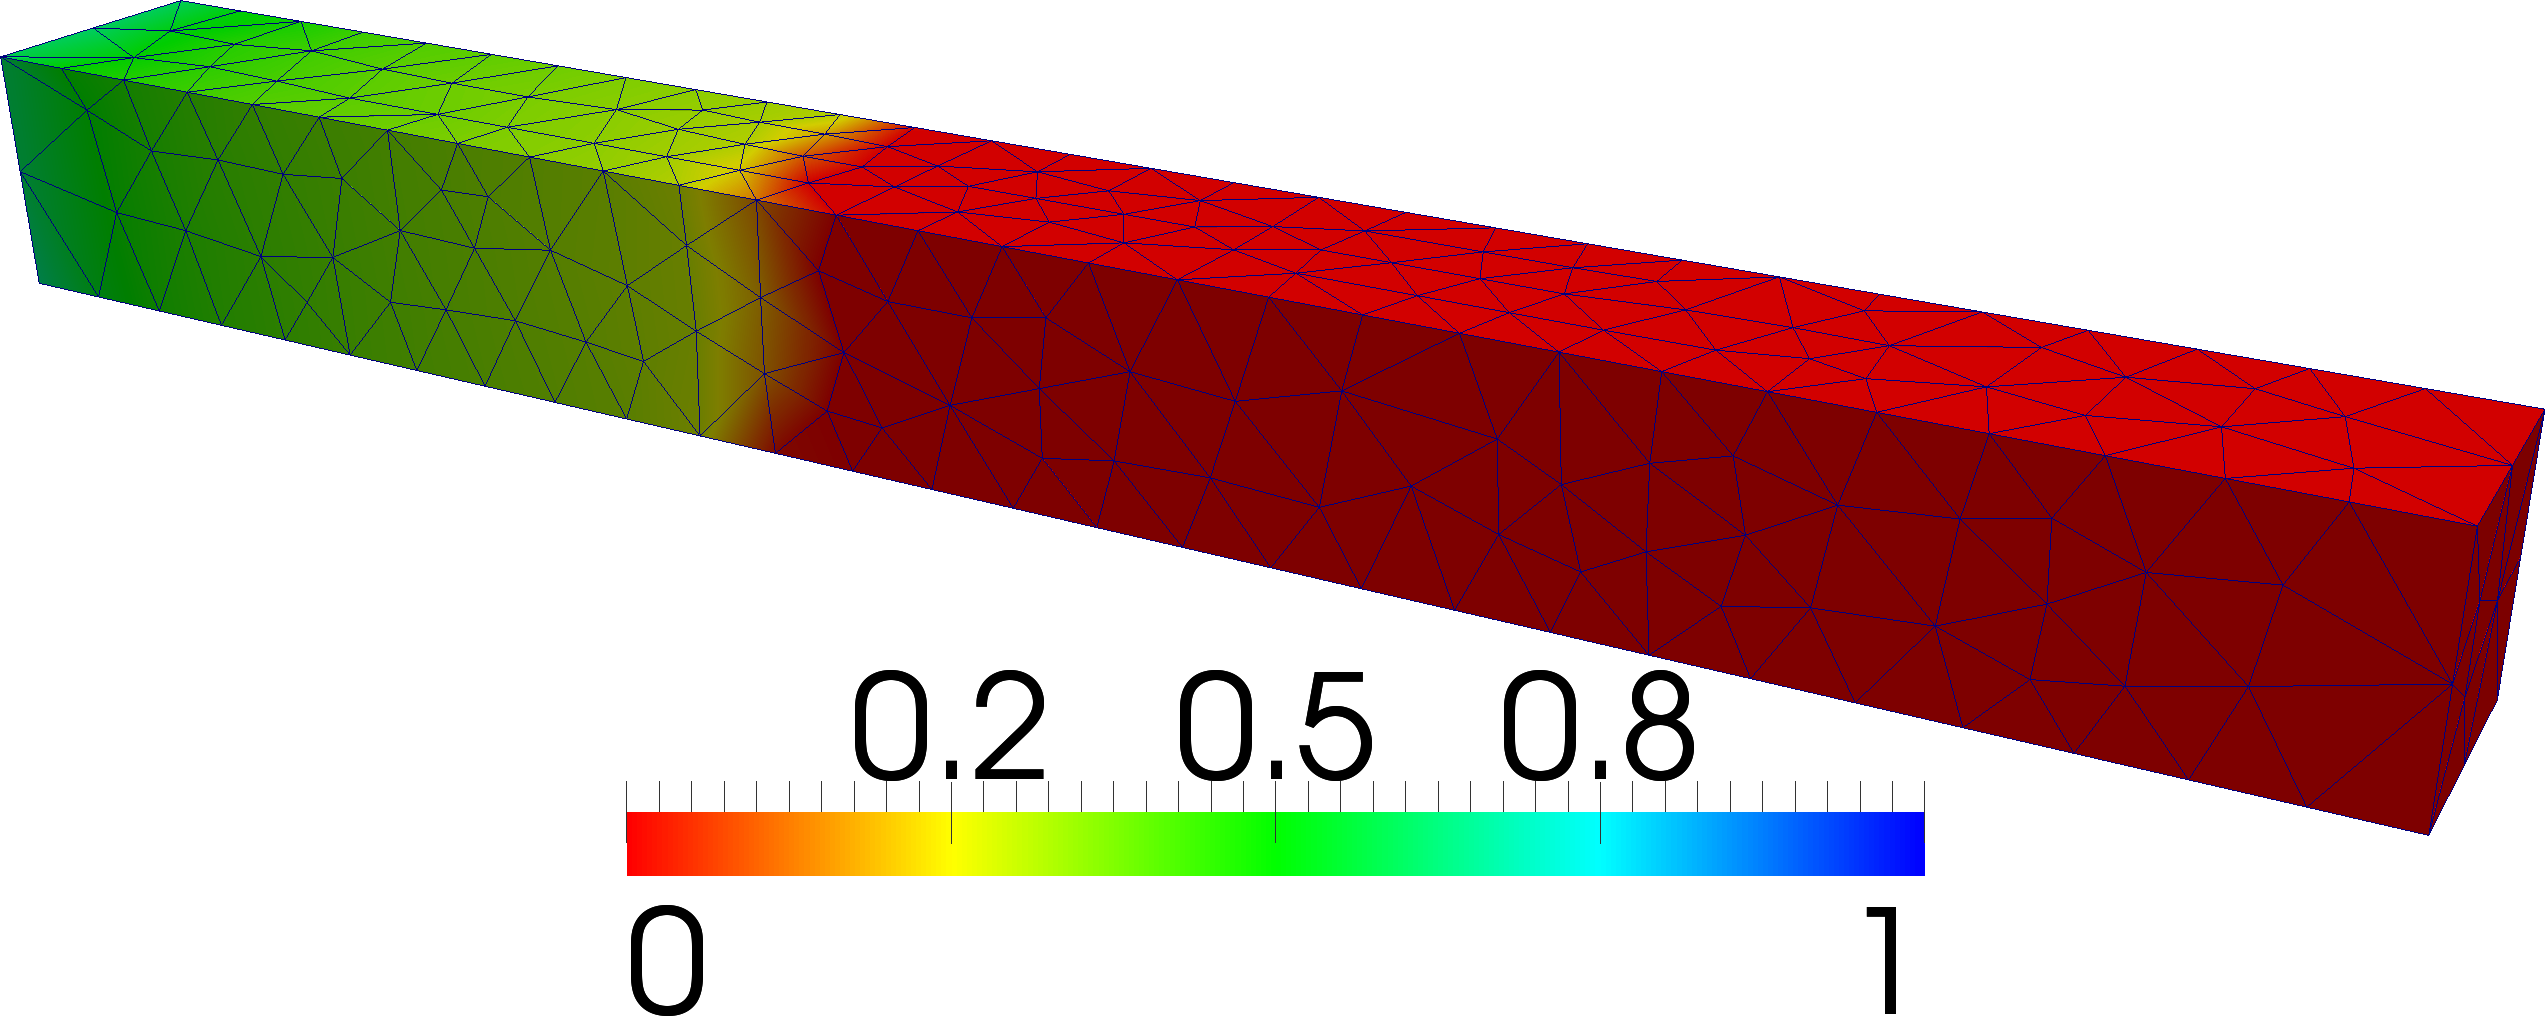
\includegraphics[width=1.\textwidth]{./diagrams/map_3d.png}}}
    \caption{Buckley-Leverett test-cases: phase 1 saturation surface maps for a 2- (770 triangles) and 3-D (1207 tetrahedra) simulations (\PN[1]{2} unstructured mesh grids) at time $t=0.5$. \label{fig:maps2d_3d}}
\end{figure}

%%%
%%%  FIGURE 
%%%
\begin{figure}[h]
\vbox{\hbox{\hspace{.3cm}
    \includegraphics[width=0.9\textwidth]{diagrams/BL_2d_P1DGP2_convergence.eps}}
\vspace{-.0cm}\hbox{\hspace{.3cm}
    \includegraphics[width=0.9\textwidth]{./diagrams/simulations_2d_3d.eps}}}
    \caption{Buckley-Leverett test-cases: 2- and 3-D phase 1 saturation profiles with \PN[1]{2} elements. Sensitivity analysis for (top) grid resolution using structured \PN[1]{2} mesh, and (bottom) mesh type.\label{fig:BL_2d_profiles}}
\end{figure}




\begin{comment}
%%%
%%%  FIGURE 
%%%
\begin{figure}[h]
\begin{center}
\includegraphics[width=1.\textwidth]{diagrams/bl-upwind-v-up-and-down.eps}
\end{center}
\caption{Buckley--Leverett test-cases: Comparison of the optimal upwind formulation when using upwinding (OU) and coupled upwind/downwind (OU-D). The finite element interpolation of the saturation field $\left(S_{1}\right)$ is shown at different mesh resolutions. Downwind seems to detract from the accuracy of the solution. \label{bl-upwind-v-up-and-down}}
\end{figure}

%%%
%%%  FIGURE 
%%%
\begin{figure}[h]
\vbox{
\begin{center}
\includegraphics[width=1.\textwidth]{diagrams/bl-exact-meth-cv-0-8-ele50.eps}
\end{center}
\vspace{0.cm}}
\caption{Buckley--Leverett test-cases: Comparison of control volume
  solutions using 80$\%$ upwinding and with optimal upwinding and
  using 50 continuous P$_{1}$DG-P$_{2}$
  elements. \label{bl-exact-meth-cv-0-8-ele50}}
\end{figure}



%%%
%%%  FIGURE 
%%%
\begin{figure}[H]
\vbox{
\begin{center}
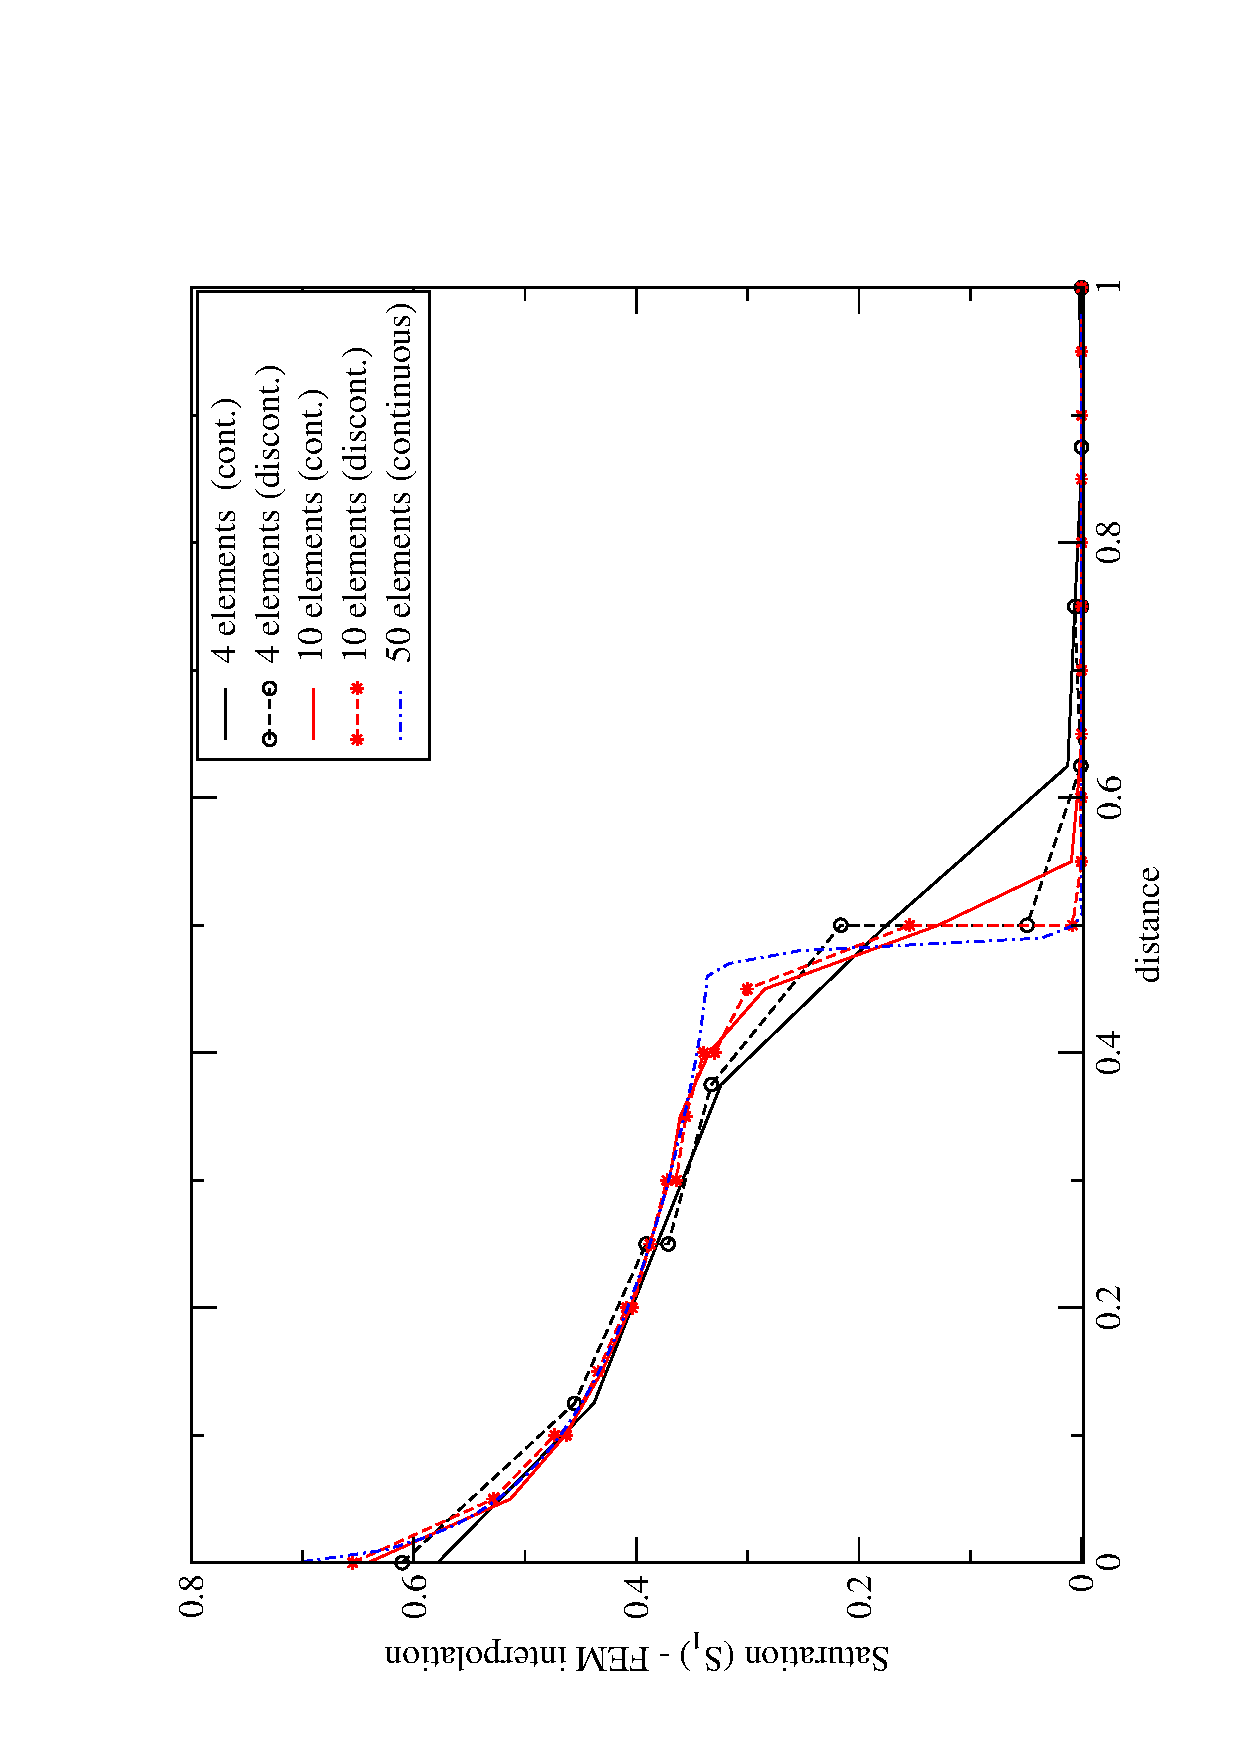
\includegraphics[width=17.5cm,height=12.5cm]{diagrams/bl-dg-4-10-vers-cty}
\end{center}
\vspace{0.cm}}
\caption{Gas saturations shown comparing the accuracy of the
  discontinuous between elements and continuous formulation. The 50
  element continuous solution may be viewed as a converged result.  }
\label{bl-dg-4-10-vers-cty}
\end{figure}

%\begin{comment}

\end{comment}

%\end{comment}
